\documentclass[12pt, a4paper, oneside]{ctexart}
\usepackage{amsmath, amsthm, amssymb, graphicx}

%导言区
\title{课程《信号与系统》笔记}
\author{NH5}
\date{更新于2025.3.9}

\begin{document}
\maketitle

\section{信号和系统的概念与分类}
\subsection{信号的分类}
信号可以从如下四个维度进行分类:

确定与随机、连续与离散、周期与非周期、能量与功率

\subsubsection{确定与随机}
\textbf{确定信号}:具有确定时间函数的信号

\textbf{随机信号}:不具有确定性函数,只能从统计意义上描述

\subsubsection{连续与离散}
连续信号和离散信号的区别在于定义域是否连续,类似函数和数列

\subsubsection{周期与非周期}
含义类似周期函数或周期数列

\textbf{注意:两个周期数列的组合不一定是周期数列}

例如:
\begin{align*}
    f_1(t) &= \cos (t)\\
    f_2(t) &= \cos (0.1 \pi t)\\
    f(t) &= f_1(t) + f_2(t)
\end{align*}

\subsubsection{能量与功率}
信号的能量与功率通过如下公式计算:

能量:
\begin{align*}
    W &= \lim_{T \to \infty}\int_{-T}^{T} |f(t)|^2 dt\\
    W &= \lim_{N \to \infty}\sum_{-N}^{N}|f(k)|^2
\end{align*}

功率:
\begin{align*}
    P &= \lim_{T \to \infty}\frac{1}{2T}\int_{-T}^{T}|f(t)|^2 dt\\
    P &= \lim_{N \to \infty}\frac{1}{2N}\sum_{-N}^{N}|f(k)|^2
\end{align*}

能量信号:
\[
    0<W<\infty,P\to 0
\]

功率信号:
\[
    0<P<\infty,W\to 0
\]

存在某些信号,既不是能量信号,也不是功率信号,例如$f(t)=e^t$.
\subsection{系统的分类}
\subsubsection{系统的定义}
系统由若干相互联系的单元组成,具有某种功能,用以达到某种目的.

激励(Excitation,$e(t)$)输入系统,输出响应(Response,$r(t)$)

\subsubsection{系统的描述}
可以通过数学模型(输入输出方程、状态方程等)或物理模型(电路等)等方式描述系统

连续时间系统用$N$阶常系数微分方程描述:
\begin{align*}
    &y^{(n)}(t)+a_{n-1}y^{(n-1)}(t)+...+a_1y^{(1)}(t)+a_0y(t)\\
    = &b_mf^{(m)}(t)+b_{m-1}f^{(m-1)}(t)+...+b_1f^{(1)}(t)+b_0f(t)
\end{align*}

方程左边是输出信号$y(t)$,方程右边是输入信号$f(t)$.

这里ppt中的公式有错误,对照教材查看是笔记当前的公式

除了微分方程,还可以用框图描述.

\subsubsection{系统的分类}
系统分类由五个维度:连续时间和离散时间、线性和非线性、时变和时不变、因果和非因果、稳定和非稳定

\textbf{连续离散}:

输入输出都是连续信号的系统是连续时间系统,相应的可以得到离散时间系统的定义

\textbf{线性非线性}:

符合\textbf{齐次性}和\textbf{叠加性}的系统是线性系统

任何线性系统都可以分解为零输入相应与零状态响应的和

\textbf{时变时不变}:

当输入从$f(t)$变为$f(t-t_0)$时,相应的输出由$y(t)$变为$y(t-t_0)$,这样的系统称为时不变系统

相应的,不满足条件的称为时变系统

\textbf{因果非因果}:

响应不早于激励产生的系统称为因果系统

可以通过判断输出是否早于输入判断系统类型

\textbf{稳定非稳定}:

对任何有界输入都只产生有界输出的系统是稳定系统

课程重点在\textbf{线性时不变连续时间系统(LTI系统)}

\section{连续时间信号}
\subsection{常用信号}
\subsubsection{正弦信号}
\[f(t)=A\sin (\omega_0t+\varphi)\]

\subsubsection{实指数信号}
\[f(t)=Ke^{\alpha t}\]
单边指数信号:
\[
    f(t)=\begin{cases}
        e^{\alpha t},&t \ge 0\\
        0,&t < 0
    \end{cases}
\]

\subsubsection{虚指数信号}
\[f(t)=e^{j\omega t}\]

它是周期信号

\subsubsection{复指数信号}
\[f(t)=Ke^{st},s=\sigma +j\omega \]

\subsubsection{抽样信号}
抽样函数具有如下性质:

实函数、偶函数、衰减函数;

零点:$x=\pm k\pi$;

最大值:$Sa(0)=1$;

\[
    \int_{-\infty}^{\infty}Sa(t)dt=\pi
\]
\begin{figure}[htbp]
    \centering
    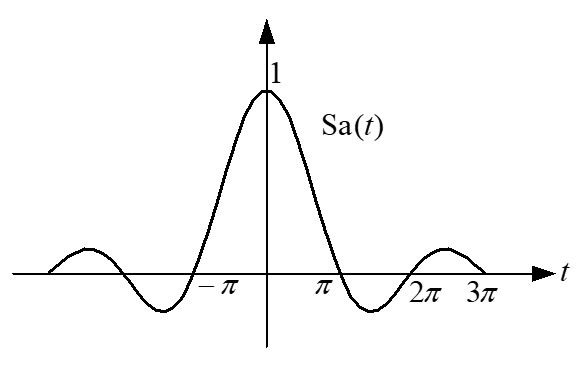
\includegraphics[width=8cm]{抽样函数.jpg}
\end{figure}

\end{document}